\documentclass{beamer}

%
% Common preamble for all three parts.
%

\usetheme[block=fill]{metropolis}
\setbeamercolor{frametitle}{use=normal text, parent=normal text}

\usepackage{arevmath}
\SetSymbolFont{largesymbols}{normal}{OMX}{iwona}{m}{n}
\usepackage{fontspec}
\setmainfont{PT Sans}
\setsansfont{PT Sans}
\setmonofont{PT Mono}[Scale=0.87]
\usepackage[english,russian]{babel}
\usepackage{amsmath}
\usepackage{color}
\usepackage{minted}
\usepackage{hyperref}
\usepackage{multicol}
\usepackage{tabularx}
\usepackage{tikz}
\usepackage{tcolorbox}

% For slide 28 (Tikz examples)
\usetikzlibrary{mindmap,trees}
\usetikzlibrary{backgrounds,shapes,arrows,positioning,calc,snakes,fit}
\usepgflibrary{decorations.markings}

\hypersetup{unicode=true}

\tcbuselibrary{skins}
\tcbuselibrary{listings}
\tcbuselibrary{minted}
\tcbset{colframe=mDarkTeal, colback=white!90!mDarkTeal,% Taken from the Metropolis theme
        left=0.8em,right=0.8em}
\newtcolorbox{tblock}[1]{boxsep=1mm,sidebyside=false,bicolor=false,colback=white,title={#1}}
\newtcolorbox{printout}{boxsep=0mm,sidebyside=false,bicolor=false,colback=white}
\def\linkbox#1{\tcbox[on line,boxsep=0mm,left=2pt,right=2pt,top=2pt,bottom=2pt,
                      colback=mDarkTeal,coltext=white]{#1}}
\def\ovllink#1{\tcbox[on line,boxsep=0mm,left=2pt,right=2pt,top=2pt,bottom=2pt,
                      colback=green!30!black,colframe=green!30!black,coltext=white]{#1}}
\newtcblisting{code}{boxsep=0mm,listing only,minted language=latex}
\newtcblisting{bibtexcode}{boxsep=0mm,listing only,minted language=bibtex}
\newtcblisting{exampletwoup}{fontupper=\small,fontlower=\small,
                             boxsep=0mm,listing side text,minted language=latex,
                             bicolor,colbacklower=white,
                             righthand ratio=0.42}
\newtcblisting{exampletwouptiny}{fontupper=\footnotesize,fontlower=\footnotesize,
                                 boxsep=0mm,listing side text,minted language=latex,
                                 minted options={fontsize=\footnotesize},
                                 bicolor,colbacklower=white,
                                 righthand ratio=0.42}
\newtcblisting{exampletwouppaused}{fontupper=\footnotesize,fontlower=\footnotesize,
                             boxsep=0mm,listing side text,minted language=latex,
                             minted options={fontsize=\footnotesize},
                             bicolor,colbacklower=white,
                             righthand ratio=0.42,after lower=\onslide<1->}
\newtcbinputlisting{\inputcode}[2][]{%
listing file={#2},boxsep=0mm,listing only,minted language=latex,#1}
\newtcbinputlisting{\inputbibtexcode}[2][]{%
listing file={#2},boxsep=0mm,listing only,minted language=bibtex,#1}

% only inline todonotes work
\usepackage{xkeyval}
\usepackage[textsize=small]{todonotes}
\presetkeys{todonotes}{inline}{}

\usetikzlibrary{shapes,arrows,positioning,shadows}

% no nav buttons
\usenavigationsymbolstemplate{}

\newcommand{\bftt}[1]{\textbf{\texttt{#1}}}
%\newcommand{\comment}[1]{{\color[HTML]{008080}\textit{\textbf{\texttt{#1}}}}}
\newcommand{\cmd}[1]{{\color[HTML]{008000}\bftt{#1}}}
\newcommand{\bs}{\char`\\}
\newcommand{\cmdbs}[1]{\cmd{\bs#1}}
\newcommand{\lcb}{\char '173}
\newcommand{\rcb}{\char '175}
\newcommand{\cmdbegin}[1]{\cmdbs{begin\lcb}\bftt{#1}\cmd{\rcb}}
\newcommand{\cmdend}[1]{\cmdbs{end\lcb}\bftt{#1}\cmd{\rcb}}

\newcommand{\wllogo}{\textbf{Overleaf}}

% this is where the example source files are loaded from
% do not include a trailing slash
\newcommand{\fileuri}{https://raw.github.com/sgolovan/latex-course/master/ru}

\newcommand{\wlserver}{https://www.overleaf.com}
\newcommand{\wlnewdoc}[1]{\wlserver/docs?snip\_uri=\fileuri/#1\&splash=none}

\def\tikzname{Ti\emph{k}Z}

% from http://tex.stackexchange.com/questions/5226/keyboard-font-for-latex
\newcommand*\keystroke[1]{%
  \tikz[baseline=(key.base)]
    \node[%
      draw,
      fill=white,
      drop shadow={shadow xshift=0.25ex,shadow yshift=-0.25ex,fill=black,opacity=0.75},
      rectangle,
      rounded corners=2pt,
      inner sep=1pt,
      line width=0.5pt,
      font=\scriptsize\ttfamily
    ](key) {#1\strut}
  ;
}
\newcommand{\keystrokebftt}[1]{\keystroke{\bftt{#1}}}

% stolen from minted.dtx
\newenvironment{exampletwouptinynoframe}
  {\VerbatimEnvironment
   \begin{VerbatimOut}{example.out}}
  {\end{VerbatimOut}
   \setlength{\parindent}{0pt}
   \begin{tabular}{l|l}
   \begin{minipage}{0.55\linewidth}
     \inputminted[fontsize=\scriptsize,resetmargins]{latex}{example.out}
   \end{minipage} &
   \begin{minipage}{0.35\linewidth}
     \setlength{\parskip}{6pt plus 1pt minus 1pt}%
     \raggedright\scriptsize\input{example.out}
   \end{minipage}
   \end{tabular}}

\title{Интерактивное введение в \LaTeX}
\author{Джон Д. Лис-Миллер\\Перевод на русский язык: Сергей Головань}
%\titlegraphic{%
%\includegraphics[height=36pt]{overleaf}\\[1em]
%\includegraphics[height=24pt]{UoB-logo}
%}


\subtitle{Часть 1: Основы}

\begin{document}

%%%%%%%%%%%%%%%%%%%%%%%%%%%%%%%%%%%%%%%%%%%%%%%%%%%%%%%%%%%%%%%%%%%%%%%%%%%%%%%
%%%%%%%%%%%%%%%%%%%%%%%%%%%%%%%%%%%%%%%%%%%%%%%%%%%%%%%%%%%%%%%%%%%%%%%%%%%%%%%
%%%%%%%%%%%%%%%%%%%%%%%%%%%%%%%%%%%%%%%%%%%%%%%%%%%%%%%%%%%%%%%%%%%%%%%%%%%%%%%
\begin{frame}
\titlepage
\end{frame}

%%%%%%%%%%%%%%%%%%%%%%%%%%%%%%%%%%%%%%%%%%%%%%%%%%%%%%%%%%%%%%%%%%%%%%%%%%%%%%%
%%%%%%%%%%%%%%%%%%%%%%%%%%%%%%%%%%%%%%%%%%%%%%%%%%%%%%%%%%%%%%%%%%%%%%%%%%%%%%%
%%%%%%%%%%%%%%%%%%%%%%%%%%%%%%%%%%%%%%%%%%%%%%%%%%%%%%%%%%%%%%%%%%%%%%%%%%%%%%%
\begin{frame}{Почему \LaTeX{}?}
\begin{itemize}
\item Он позволяет набирать красивые документы
\begin{itemize}
\item Особенно с математическими формулами
\end{itemize}
%
\item Он был создан учёными для учёных
\begin{itemize}
\item Большое и активное сообщество пользователей и разработчиков
\end{itemize}
%
\item Он мощный, вы можете расширять его
\begin{itemize}
\item Пакеты для статей, презентаций, электронных таблиц, \dots
\end{itemize}
\end{itemize}
\end{frame}

%%%%%%%%%%%%%%%%%%%%%%%%%%%%%%%%%%%%%%%%%%%%%%%%%%%%%%%%%%%%%%%%%%%%%%%%%%%%%%%
%%%%%%%%%%%%%%%%%%%%%%%%%%%%%%%%%%%%%%%%%%%%%%%%%%%%%%%%%%%%%%%%%%%%%%%%%%%%%%%
%%%%%%%%%%%%%%%%%%%%%%%%%%%%%%%%%%%%%%%%%%%%%%%%%%%%%%%%%%%%%%%%%%%%%%%%%%%%%%%
\begin{frame}[fragile]{Как он работает?}
\begin{itemize}
\item Вы набираете документ в формате \emph{обычного текста} с \cmd{командами},
  которые описывают его структуру и смысл.
\item Программа \texttt{latex} обрабатывает ваш текст и команды и преобразовывает
  его в красиво отформатированный документ.
\end{itemize}
\begin{center}
\begin{code}
Шла Саша по шоссе и сосала \emph{сушку}.
\end{code}
\tikz\node[single arrow,fill=gray,font=\ttfamily\bfseries,%
  rotate=270,xshift=-1em]{latex};
\begin{printout}
Шла Саша по шоссе и сосала \emph{сушку}.
\end{printout}
\end{center}
\end{frame}

%%%%%%%%%%%%%%%%%%%%%%%%%%%%%%%%%%%%%%%%%%%%%%%%%%%%%%%%%%%%%%%%%%%%%%%%%%%%%%%
%%%%%%%%%%%%%%%%%%%%%%%%%%%%%%%%%%%%%%%%%%%%%%%%%%%%%%%%%%%%%%%%%%%%%%%%%%%%%%%
%%%%%%%%%%%%%%%%%%%%%%%%%%%%%%%%%%%%%%%%%%%%%%%%%%%%%%%%%%%%%%%%%%%%%%%%%%%%%%%
\begin{frame}[fragile]{Ещё примеры команд и их результат\dots}
\vspace{-0.5mm}
\begin{exampletwoup}
\begin{itemize}
\item Чай
\item Молоко
\item Печенье
\end{itemize}
\end{exampletwoup}
\vspace{-0.5mm}
\begin{exampletwoup}
\begin{figure}
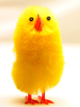
\includegraphics{chick}
\end{figure}
\end{exampletwoup}
\vspace{-0.5mm}
\begin{exampletwoup}
\begin{equation}
\alpha + \beta + 1
\end{equation}
\end{exampletwoup}
\vspace{-3mm}
\tiny{Изображение взято с \url{http://www.andy-roberts.net/writing/latex/importing_images}}
\end{frame}

%%%%%%%%%%%%%%%%%%%%%%%%%%%%%%%%%%%%%%%%%%%%%%%%%%%%%%%%%%%%%%%%%%%%%%%%%%%%%%%
%%%%%%%%%%%%%%%%%%%%%%%%%%%%%%%%%%%%%%%%%%%%%%%%%%%%%%%%%%%%%%%%%%%%%%%%%%%%%%%
%%%%%%%%%%%%%%%%%%%%%%%%%%%%%%%%%%%%%%%%%%%%%%%%%%%%%%%%%%%%%%%%%%%%%%%%%%%%%%%
\begin{frame}[fragile]{Смена подхода}

\begin{itemize}
\item Используйте команды, чтобы описывать <<что это>>, а не <<как это выглядит>>.
\item Сосредоточьтесь на содержании.
\item Позвольте \LaTeX{} делать его работу.
\end{itemize}
\end{frame}

%%%%%%%%%%%%%%%%%%%%%%%%%%%%%%%%%%%%%%%%%%%%%%%%%%%%%%%%%%%%%%%%%%%%%%%%%%%%%%%
%%%%%%%%%%%%%%%%%%%%%%%%%%%%%%%%%%%%%%%%%%%%%%%%%%%%%%%%%%%%%%%%%%%%%%%%%%%%%%%
%%%%%%%%%%%%%%%%%%%%%%%%%%%%%%%%%%%%%%%%%%%%%%%%%%%%%%%%%%%%%%%%%%%%%%%%%%%%%%%
\section{Основы}

%%%%%%%%%%%%%%%%%%%%%%%%%%%%%%%%%%%%%%%%%%%%%%%%%%%%%%%%%%%%%%%%%%%%%%%%%%%%%%%
%%%%%%%%%%%%%%%%%%%%%%%%%%%%%%%%%%%%%%%%%%%%%%%%%%%%%%%%%%%%%%%%%%%%%%%%%%%%%%%
%%%%%%%%%%%%%%%%%%%%%%%%%%%%%%%%%%%%%%%%%%%%%%%%%%%%%%%%%%%%%%%%%%%%%%%%%%%%%%%
\subsection{Первые шаги}

\begin{frame}[fragile]{\insertsubsection}
\vspace{-2ex}
\begin{itemize}
  \item Минимальный документ \LaTeX{} (на русском языке):

\inputcode{basics.tex}
\item Команды начинаются с \emph{обратной косой} \keystrokebftt{\bs}.
\item Каждый документ начинается с команды \cmdbs{documentclass}.
\item \emph{Аргумент} в фигурных скобках \keystrokebftt{\{} \keystrokebftt{\}}
  указывает \LaTeX'у что именно за документ мы пишем: \bftt{article} означает статья.
\item Значок процента \keystrokebftt{\%} начинает \emph{комментарий} --- \LaTeX{}
проигнорирует оставшуюся часть строки.
\item Пока что переносы для русского языка отключены, мы рассмотрим их во
  второй части курса
\end{itemize}
\end{frame}

%%%%%%%%%%%%%%%%%%%%%%%%%%%%%%%%%%%%%%%%%%%%%%%%%%%%%%%%%%%%%%%%%%%%%%%%%%%%%%%
%%%%%%%%%%%%%%%%%%%%%%%%%%%%%%%%%%%%%%%%%%%%%%%%%%%%%%%%%%%%%%%%%%%%%%%%%%%%%%%
%%%%%%%%%%%%%%%%%%%%%%%%%%%%%%%%%%%%%%%%%%%%%%%%%%%%%%%%%%%%%%%%%%%%%%%%%%%%%%%
\begin{frame}[fragile]{\insertsubsection{} в \wllogo}
\begin{itemize}
\item Overleaf --- это вебсайт, позволяющий набирать документы \LaTeX{} в интернете.
\item Он <<компилирует>> ваш текст \LaTeX{} автоматически и показывает результат.
\begin{center}
\ovlhref{basics.tex}{Щёлкните здесь, чтобы открыть пример документа в \wllogo{}}

\vspace{1ex}
\scriptsize
Для лучшего результата воспользуйтесь браузером
\href{http://www.google.com/chrome}{Google Chrome} или новой версией браузера
\href{http://www.mozilla.org/en-US/firefox/new/}{FireFox}.
\end{center}
\vspace{1ex}
\item В дальнейшем при просмотре слайдов пробуйте набирать рассматриваемые
  примеры в Overleaf.
\item \textbf{Нет, правда, вы должны их попробовать по мере просмотра!}
\end{itemize}
\end{frame}

%%%%%%%%%%%%%%%%%%%%%%%%%%%%%%%%%%%%%%%%%%%%%%%%%%%%%%%%%%%%%%%%%%%%%%%%%%%%%%%
%%%%%%%%%%%%%%%%%%%%%%%%%%%%%%%%%%%%%%%%%%%%%%%%%%%%%%%%%%%%%%%%%%%%%%%%%%%%%%%
%%%%%%%%%%%%%%%%%%%%%%%%%%%%%%%%%%%%%%%%%%%%%%%%%%%%%%%%%%%%%%%%%%%%%%%%%%%%%%%
\subsection{Набор текста}
\begin{frame}[fragile]{\insertsubsection{}}
\small
\begin{itemize}
\item Набирайте ваш текст между \cmdbegin{document} и \cmdend{document}.
\item По большей части вы можете просто вводить текст как есть.

\begin{exampletwouptiny}
Слова разделяются одним
пробелом или несколькими.

Абзацы разделяются одной
пустой строкой или
несколькими.
\end{exampletwouptiny}
\item Несколько пробелов подряд в исходном тексте воспринимаются как один.

\begin{exampletwouptiny}
Шла     Саша    по  шоссе
и      сосала      сушку.
\end{exampletwouptiny}
\end{itemize}
\end{frame}

%%%%%%%%%%%%%%%%%%%%%%%%%%%%%%%%%%%%%%%%%%%%%%%%%%%%%%%%%%%%%%%%%%%%%%%%%%%%%%%
%%%%%%%%%%%%%%%%%%%%%%%%%%%%%%%%%%%%%%%%%%%%%%%%%%%%%%%%%%%%%%%%%%%%%%%%%%%%%%%
%%%%%%%%%%%%%%%%%%%%%%%%%%%%%%%%%%%%%%%%%%%%%%%%%%%%%%%%%%%%%%%%%%%%%%%%%%%%%%%
\begin{frame}[fragile]{\insertsubsection{}: особенности}
\vspace{-3ex}
\small
\begin{itemize}
\item Символы кавычек вводятся хитро: используются символы \keystroke{<} и
  \keystroke{>} для <<ёлочек>>, и запятая \keystroke{,} с обратной кавычкой
  \keystroke{\char96} для ,,лапок``.
\begin{exampletwouptiny}
Кавычки-ёлочки: <<текст>>.

Кавычки-лапки: ,,текст``.
\end{exampletwouptiny}
\item Некоторые часто встречающиеся символы имеют специальный смысл в \LaTeX:

\begin{tabular}{cl}
\keystrokebftt{\%} & значок процента     \\
\keystrokebftt{\#} & значок диеза / хэша \\
\keystrokebftt{\&} & амперсанд           \\
\keystrokebftt{\$} & значок доллара      \\
\end{tabular}
\item Если ввести эти символы непосредственно, то получится ошибка. Если
  нужно, чтобы эти значки появились в документе, то их придётся \emph{экранировать}
  с помощью обратной косой.
\begin{exampletwoup}
\$\%\&\#!
\end{exampletwoup}
\end{itemize}
\end{frame}

%%%%%%%%%%%%%%%%%%%%%%%%%%%%%%%%%%%%%%%%%%%%%%%%%%%%%%%%%%%%%%%%%%%%%%%%%%%%%%%
%%%%%%%%%%%%%%%%%%%%%%%%%%%%%%%%%%%%%%%%%%%%%%%%%%%%%%%%%%%%%%%%%%%%%%%%%%%%%%%
%%%%%%%%%%%%%%%%%%%%%%%%%%%%%%%%%%%%%%%%%%%%%%%%%%%%%%%%%%%%%%%%%%%%%%%%%%%%%%%
\begin{frame}[fragile]{\insertsubsection{}: особенности}
\vspace{-2ex}
\small
Следует также отметить, что в печатной продукции встречаются четыре
вида <<тире>>. В \LaTeX{} они вводятся специальным образом:
\vspace{-1ex}
\begin{description}
  \item[\keystrokebftt{-}] дефис
  \item[\keystrokebftt{-}\keystrokebftt{-}] короткое тире, используется
    при перечислении или задании диапазонов
  \item[\keystrokebftt{-}\keystrokebftt{-}\keystrokebftt{-}] длинное тире,
    используется в прямой речи или как собственно тире в тексте
  \item[\keystrokebftt{\$}\keystrokebftt{-}\keystrokebftt{\$}] минус в
    математическом режиме, $x - y$
\end{description}
\begin{exampletwouptiny}
Бело-голубые цвета.

Теорема Гаусса--Маркова. стр. 2--6.

Единица --- ноль!

$2 - 1 = 0$.
\end{exampletwouptiny}
\end{frame}

%%%%%%%%%%%%%%%%%%%%%%%%%%%%%%%%%%%%%%%%%%%%%%%%%%%%%%%%%%%%%%%%%%%%%%%%%%%%%%%
%%%%%%%%%%%%%%%%%%%%%%%%%%%%%%%%%%%%%%%%%%%%%%%%%%%%%%%%%%%%%%%%%%%%%%%%%%%%%%%
%%%%%%%%%%%%%%%%%%%%%%%%%%%%%%%%%%%%%%%%%%%%%%%%%%%%%%%%%%%%%%%%%%%%%%%%%%%%%%%
\begin{frame}[fragile]{Работа над ошибками}
\vspace{-3ex}
\small
\begin{itemize}
\item Иногда \LaTeX{} не может скомпилировать ваш документ. В этом случае он
останавливается и выдаёт сообщение об ошибке, которую вам нужно исправить,
иначе результата не добиться.
\item Например, если вы ошиблись в написании команды \cmdbs{emph} и получили
\cmdbs{meph}, \LaTeX{} остановится с ошибкой <<undefined control sequence>>,
потому что он не знаком с командой \cmdbs{meph}.
\end{itemize}
\vspace{-1ex}
\begin{tblock}{Советы по работе с ошибками}
\begin{enumerate}
\item Не паниковать! Ошибки бывают у всех.
\item Исправлять их следует сразу же после обнаружения --- если только что написанный
текст вызвал ошибку, можно начать отладку с него.
\item Если проявилось несколько ошибок сразу, начинайте исправлять с самой первой ---
на самом деле проблема может быть еще выше по тексту.
\end{enumerate}
\end{tblock}
\end{frame}

%%%%%%%%%%%%%%%%%%%%%%%%%%%%%%%%%%%%%%%%%%%%%%%%%%%%%%%%%%%%%%%%%%%%%%%%%%%%%%%
%%%%%%%%%%%%%%%%%%%%%%%%%%%%%%%%%%%%%%%%%%%%%%%%%%%%%%%%%%%%%%%%%%%%%%%%%%%%%%%
%%%%%%%%%%%%%%%%%%%%%%%%%%%%%%%%%%%%%%%%%%%%%%%%%%%%%%%%%%%%%%%%%%%%%%%%%%%%%%%
\begin{frame}[fragile]{Упражнение наборщика 1}

\begin{tblock}{Наберите этот текст в \LaTeX:\footnotemark}
По итогам 2015 года ВВП России снизился (на 2.8\%), впервые после кризиса
2008--2009 годов. Инфляция выросла до 12.9\%. Реальные доходы населения
снизились на 3.2\%. В то же время произошло снижение оттока капитала почти в
3 раза (до \$58 млрд).
\end{tblock}
\footnotetext{\href{https://ru.wikipedia.org/wiki/\%D0\%AD\%D0\%BA\%D0\%BE\%D0\%BD\%D0\%BE\%D0\%BC\%D0\%B8\%D0\%BA\%D0\%B0_\%D0\%A0\%D0\%BE\%D1\%81\%D1\%81\%D0\%B8\%D0\%B8}{https://ru.wikipedia.org/wiki/Экономика\_{}России}}
\vskip 1ex
\begin{center}
\ovlhref{basics-exercise-1.tex}{Щёлкните, чтобы открыть это упражнение в \wllogo{}}
\end{center}
\begin{itemize}
\item Указание: обращайте внимание на специальные символы!
\item Когда попробуете,
\ovlhref{basics-exercise-1-solution.tex}{щёлкните, чтобы посмотреть решение}.
\vspace{2ex}
\end{itemize}
\end{frame}

%%%%%%%%%%%%%%%%%%%%%%%%%%%%%%%%%%%%%%%%%%%%%%%%%%%%%%%%%%%%%%%%%%%%%%%%%%%%%%%
%%%%%%%%%%%%%%%%%%%%%%%%%%%%%%%%%%%%%%%%%%%%%%%%%%%%%%%%%%%%%%%%%%%%%%%%%%%%%%%
%%%%%%%%%%%%%%%%%%%%%%%%%%%%%%%%%%%%%%%%%%%%%%%%%%%%%%%%%%%%%%%%%%%%%%%%%%%%%%%
\subsection{Набор математики}

\begin{frame}[fragile]{\insertsubsection{}: Значки доллара}
\begin{itemize}
\item Что такого особенного в значках доллара \keystrokebftt{\$}, Они применяются
для переключения в математический режим в тексте.\\[1ex]
\begin{exampletwouptiny}
% результат так себе:
Пусть a и b --- два разных
натуральных числа и пусть
c = a - b + 1.

% так намного лучше:
Пусть $a$ и $b$ --- два разных
натуральных числа и пусть
$c = a - b + 1$.
\end{exampletwouptiny}
\item Всегда ставьте знаки доллара парами --- один чтобы начать математической
  формулы, другой чтобы её закончить.
\end{itemize}
\end{frame}

%%%%%%%%%%%%%%%%%%%%%%%%%%%%%%%%%%%%%%%%%%%%%%%%%%%%%%%%%%%%%%%%%%%%%%%%%%%%%%%
%%%%%%%%%%%%%%%%%%%%%%%%%%%%%%%%%%%%%%%%%%%%%%%%%%%%%%%%%%%%%%%%%%%%%%%%%%%%%%%
%%%%%%%%%%%%%%%%%%%%%%%%%%%%%%%%%%%%%%%%%%%%%%%%%%%%%%%%%%%%%%%%%%%%%%%%%%%%%%%
\begin{frame}[fragile]{\insertsubsection{}: Особенности}
\begin{itemize}
\item \LaTeX{} расставляет пробелы в математическом режиме самостоятельно, он
  игнорирует пробелы, которые вы поставили.

\vspace{2pt}
\begin{exampletwouptiny}
Пусть $y=mx+b$ --- \dots

Пусть $y = m x + b$ --- \dots
\end{exampletwouptiny}

\item Используйте <<крышку>> \keystrokebftt{\char94} для верхних индексов и
  подчёркивание \keystrokebftt{\_} для нижних.

\vspace{2pt}
\begin{exampletwouptiny}
$y = c_2 x^2 + c_1 x + c_0$
\end{exampletwouptiny}
\end{itemize}
\end{frame}

%%%%%%%%%%%%%%%%%%%%%%%%%%%%%%%%%%%%%%%%%%%%%%%%%%%%%%%%%%%%%%%%%%%%%%%%%%%%%%%
%%%%%%%%%%%%%%%%%%%%%%%%%%%%%%%%%%%%%%%%%%%%%%%%%%%%%%%%%%%%%%%%%%%%%%%%%%%%%%%
%%%%%%%%%%%%%%%%%%%%%%%%%%%%%%%%%%%%%%%%%%%%%%%%%%%%%%%%%%%%%%%%%%%%%%%%%%%%%%%
\begin{frame}[fragile]{\insertsubsection{}: Обозначения}
\begin{itemize}
\item Используйте фигурные скобки \keystrokebftt{\{} \keystrokebftt{\}} для
группировки верхних и нижних индексов.

\begin{exampletwouptiny}
$F_n = F_n-1 + F_n-2$ % ой!

$F_n = F_{n-1} + F_{n-2}$
\end{exampletwouptiny}

\item Греческие буквы и математические операции набираются с помощью команд
  с говорящими именами.

\begin{exampletwouptiny}
$\mu = A e^{Q/RT}$

$\Omega =
  \sum_{k=1}^{n} \omega_k$
\end{exampletwouptiny}
\end{itemize}
\end{frame}

%%%%%%%%%%%%%%%%%%%%%%%%%%%%%%%%%%%%%%%%%%%%%%%%%%%%%%%%%%%%%%%%%%%%%%%%%%%%%%%
%%%%%%%%%%%%%%%%%%%%%%%%%%%%%%%%%%%%%%%%%%%%%%%%%%%%%%%%%%%%%%%%%%%%%%%%%%%%%%%
%%%%%%%%%%%%%%%%%%%%%%%%%%%%%%%%%%%%%%%%%%%%%%%%%%%%%%%%%%%%%%%%%%%%%%%%%%%%%%%
\begin{frame}[fragile]{\insertsubsection{}: Выключные уравнения}
\begin{itemize}
  \item Если уравнение большое и страшное, \emph{вынесите} его на отдельную
    строку с помощью
\cmdbegin{equation} и \cmdend{equation}.
\vspace{1ex}
\begin{exampletwouptiny}
Корни квадратного уравнения
можно найти по формуле
\begin{equation}
x =
\frac{-b \pm\sqrt{b^2 - 4ac}}
     {2a}
\end{equation}
где $a$, $b$ и $c$ --- \dots
\end{exampletwouptiny}

{\scriptsize Замечание: \LaTeX{} почти всегда игнорирует пробелы при наборе
  математики, но пустые строки он воспринимает как ошибки --- не вставляйте
  пустые строки в формулы.}
\end{itemize}
\end{frame}

%%%%%%%%%%%%%%%%%%%%%%%%%%%%%%%%%%%%%%%%%%%%%%%%%%%%%%%%%%%%%%%%%%%%%%%%%%%%%%%
%%%%%%%%%%%%%%%%%%%%%%%%%%%%%%%%%%%%%%%%%%%%%%%%%%%%%%%%%%%%%%%%%%%%%%%%%%%%%%%
%%%%%%%%%%%%%%%%%%%%%%%%%%%%%%%%%%%%%%%%%%%%%%%%%%%%%%%%%%%%%%%%%%%%%%%%%%%%%%%
\begin{frame}[fragile]{Отступление: Окружения}
\begin{itemize}
\item \bftt{equation} это \emph{окружение}, оно задаёт контекст.
\item Одна и та же команда может выводить разный результат в разном контексте.

\begin{exampletwouptiny}
Можно писать
$\Omega=\sum_{k=1}^{n}\omega_k$
в тексте, а можно писать
\begin{equation}
  \Omega=\sum_{k=1}^{n}\omega_k
\end{equation}
в отдельной строке.
\end{exampletwouptiny}
\vspace{1ex}
\item Видите, как $\Sigma$ увеличилась в окружении \bftt{equation}, а также,
как переместились верхние и нижние индексы, а ведь использовалась та же команда.
\vskip 1ex
{\scriptsize В принципе, можно было бы писать \bftt{\$...\$} как
\cmdbegin{math}\bftt{...}\cmdend{math}.}
\end{itemize}
\end{frame}

%%%%%%%%%%%%%%%%%%%%%%%%%%%%%%%%%%%%%%%%%%%%%%%%%%%%%%%%%%%%%%%%%%%%%%%%%%%%%%%
%%%%%%%%%%%%%%%%%%%%%%%%%%%%%%%%%%%%%%%%%%%%%%%%%%%%%%%%%%%%%%%%%%%%%%%%%%%%%%%
%%%%%%%%%%%%%%%%%%%%%%%%%%%%%%%%%%%%%%%%%%%%%%%%%%%%%%%%%%%%%%%%%%%%%%%%%%%%%%%
\begin{frame}[fragile]{Отступление: Окружения}
\begin{itemize}
\item Команды \cmdbs{begin} и \cmdbs{end} используются для создания разных
  окружений.

\item Окружения \bftt{itemize} и \bftt{enumerate} печатают списки.
\vskip 1ex

\begin{exampletwouptiny}
% ненумерованный список
\begin{itemize}
\item Печенье
\item Чай
\end{itemize}

%нумерованный список
\begin{enumerate}
\item Печенье
\item Чай
\end{enumerate}
\end{exampletwouptiny}
\end{itemize}
\end{frame}

%%%%%%%%%%%%%%%%%%%%%%%%%%%%%%%%%%%%%%%%%%%%%%%%%%%%%%%%%%%%%%%%%%%%%%%%%%%%%%%
%%%%%%%%%%%%%%%%%%%%%%%%%%%%%%%%%%%%%%%%%%%%%%%%%%%%%%%%%%%%%%%%%%%%%%%%%%%%%%%
%%%%%%%%%%%%%%%%%%%%%%%%%%%%%%%%%%%%%%%%%%%%%%%%%%%%%%%%%%%%%%%%%%%%%%%%%%%%%%%
\begin{frame}[fragile]{Отступление: Пакеты}
\vspace{-3ex}
\begin{itemize}
  \item Все команды и окружения, которые мы до сих пор
    использовали,\footnote{Кроме \cmdbs{setmainfont} при подключении шрифта
    с русскими буквами} были встроены в \LaTeX.

\item \emph{Пакеты} это библиотеки дополнительных команд и окружений.
  Существуют тысячи пакетов в свободном доступе.

\item Чтобы загрузить пакет и пользоваться реализованными в нём командами,
  нужно использовать команду \cmdbs{usepackage} в \emph{преамбуле}.

\item Пример: \bftt{amsmath} от Американского математического общества.
\begin{code}
\documentclass{article}
\usepackage{amsmath} % преамбула
\begin{document}
% теперь можно использовать команды из amsmath...
\end{document}
\end{code}
\vspace*{2pt}
\end{itemize}
\end{frame}

%%%%%%%%%%%%%%%%%%%%%%%%%%%%%%%%%%%%%%%%%%%%%%%%%%%%%%%%%%%%%%%%%%%%%%%%%%%%%%%
%%%%%%%%%%%%%%%%%%%%%%%%%%%%%%%%%%%%%%%%%%%%%%%%%%%%%%%%%%%%%%%%%%%%%%%%%%%%%%%
%%%%%%%%%%%%%%%%%%%%%%%%%%%%%%%%%%%%%%%%%%%%%%%%%%%%%%%%%%%%%%%%%%%%%%%%%%%%%%%
\begin{frame}[fragile]{\insertsubsection{}: Примеры с \bftt{amsmath}}
\vspace{-2ex}
\begin{itemize}
\item Можно использовать \bftt{equation*} (<<equation со звёздочкой>>) для
  уравнений без номера.
\begin{exampletwouptiny}
\begin{equation*}
\Omega=\sum_{k=1}^{n}\omega_k
\end{equation*}
\end{exampletwouptiny}
\item \LaTeX{} трактует рядом стоящие буквы как отдельные переменные, и это
  не всегда то, что хочется. В \bftt{amsmath} определены команды для многих
  часто используемых математических операторов.
\begin{exampletwouptiny}
\begin{equation*} % плохо!
 min_{x,y}(1-x)^2+10(y-x^2)^2
\end{equation*}
\begin{equation*} % хорошо!
\min_{x,y}(1-x)^2+10(y-x^2)^2
\end{equation*}
\end{exampletwouptiny}
\end{itemize}
\end{frame}

%%%%%%%%%%%%%%%%%%%%%%%%%%%%%%%%%%%%%%%%%%%%%%%%%%%%%%%%%%%%%%%%%%%%%%%%%%%%%%%
%%%%%%%%%%%%%%%%%%%%%%%%%%%%%%%%%%%%%%%%%%%%%%%%%%%%%%%%%%%%%%%%%%%%%%%%%%%%%%%
%%%%%%%%%%%%%%%%%%%%%%%%%%%%%%%%%%%%%%%%%%%%%%%%%%%%%%%%%%%%%%%%%%%%%%%%%%%%%%%
\begin{frame}[fragile]{\insertsubsection{}: Примеры с \bftt{amsmath}}
\vspace{-2ex}
\begin{itemize}
\item Если подходящего оператора не нашлось, можно воспользоваться \cmdbs{operatorname}.
\vspace{1ex}
\begin{exampletwouptiny}
\begin{equation*}
\beta_i =
\frac
  {\operatorname{Cov}(R_i,R_m)}
  {\operatorname{Var}(R_m)}
\end{equation*}
\end{exampletwouptiny}
\end{itemize}
\end{frame}

%%%%%%%%%%%%%%%%%%%%%%%%%%%%%%%%%%%%%%%%%%%%%%%%%%%%%%%%%%%%%%%%%%%%%%%%%%%%%%%
%%%%%%%%%%%%%%%%%%%%%%%%%%%%%%%%%%%%%%%%%%%%%%%%%%%%%%%%%%%%%%%%%%%%%%%%%%%%%%%
%%%%%%%%%%%%%%%%%%%%%%%%%%%%%%%%%%%%%%%%%%%%%%%%%%%%%%%%%%%%%%%%%%%%%%%%%%%%%%%
\begin{frame}[fragile]{\insertsubsection{}: Примеры с \bftt{amsmath}}
\vspace{-2ex}
\begin{itemize}{\small
\item Можно выравнивать несколько уравнений по знакам равенства
\begin{printout}
\vspace{-2.5ex}
\begin{align*}
(x+1)^3 &= (x+1)(x+1)(x+1) \\
        &= (x+1)(x^2 + 2x + 1) \\
        &= x^3 + 3x^2 + 3x + 1
\end{align*}
\end{printout}
с помощью окружения \bftt{align*}.

\vspace{1ex}
% for whatever reason, this doesn't play well with the twoup environment
\begin{code}
\begin{align*}
(x+1)^3 &= (x+1)(x+1)(x+1) \\
        &= (x+1)(x^2 + 2x + 1) \\
        &= x^3 + 3x^2 + 3x + 1
\end{align*}
\end{code}
\item Символ амперсанда \keystrokebftt{\&} отделяет левую колонку (до знака
  $=$) от правой колонки (после знака $=$).
\item Двойной обратной косой \keystrokebftt{\bs}\keystrokebftt{\bs} начинает
  новую строку.
}\end{itemize}
\end{frame}


%%%%%%%%%%%%%%%%%%%%%%%%%%%%%%%%%%%%%%%%%%%%%%%%%%%%%%%%%%%%%%%%%%%%%%%%%%%%%%%
%%%%%%%%%%%%%%%%%%%%%%%%%%%%%%%%%%%%%%%%%%%%%%%%%%%%%%%%%%%%%%%%%%%%%%%%%%%%%%%
%%%%%%%%%%%%%%%%%%%%%%%%%%%%%%%%%%%%%%%%%%%%%%%%%%%%%%%%%%%%%%%%%%%%%%%%%%%%%%%
\begin{frame}[fragile]{Упражнение наборщика 2}
\vspace{-1.5ex}
\abovedisplayskip=1pt
\belowdisplayskip=1pt
\begin{tblock}{Наберите этот текст в \LaTeX:}
Пусть $X_1, X_2, \dots, X_n$ --- последовательность независимых одинаково
распределённых случайных величин, для которых
$\operatorname{E}[X_i] = \mu$ и
$\operatorname{Var}[X_i] = \sigma^2 < \infty$, и пусть
\begin{equation*}
S_n = \frac{1}{n}\sum_{i=1}^{n} X_i
\end{equation*}
обозначает их среднее арифметическое. Тогда при $n$, стремящемся к
бесконечности, последовательность случайных величин
$\sqrt{n}(S_n - \mu)$ сходится по распределению к нормальной $N(0, \sigma^2)$
величине.
\end{tblock}
\vspace{-0.5ex}
\begin{center}
\ovlhref{basics-exercise-2.tex}{Щёлкните, чтобы открыть это упражнение в \wllogo{}}
\end{center}
\vspace{-2ex}
\begin{itemize}
\item Указание: Символ $\infty$ набирается как \cmdbs{infty}.
\item Когда попробуете,
\ovlhref{basics-exercise-2-solution.tex}{щёлкните, чтобы посмотреть решение}.
\end{itemize}
\end{frame}

%%%%%%%%%%%%%%%%%%%%%%%%%%%%%%%%%%%%%%%%%%%%%%%%%%%%%%%%%%%%%%%%%%%%%%%%%%%%%%%
%%%%%%%%%%%%%%%%%%%%%%%%%%%%%%%%%%%%%%%%%%%%%%%%%%%%%%%%%%%%%%%%%%%%%%%%%%%%%%%
%%%%%%%%%%%%%%%%%%%%%%%%%%%%%%%%%%%%%%%%%%%%%%%%%%%%%%%%%%%%%%%%%%%%%%%%%%%%%%%
\begin{frame}{Конец первой части}
\begin{itemize}
\item Поздравляем! Вы уже узнали, как \dots
\begin{itemize}
\item Набирать текст в \LaTeX.
\item Использовать множество разных команд.
\item Исправлять ошибки, когда они возникают.
\item Красиво набирать математические формулы.
\item Пользоваться несколькими различными окружениями.
\item Подключать пакеты.
\end{itemize}
\item Это уже немало!
\item Во второй части вы увидите, как, используя \LaTeX{}, набирать
  структурированные документы с разделами, перекрёстными ссылками,
  рисунками, таблицами и списком литературы. До встречи!
\end{itemize}
\end{frame}

\end{document}
